\documentclass[12pt]{report}
\usepackage[utf8]{inputenc}
\usepackage{geometry}
 \geometry{
 a4paper,
 total={210mm,297mm},
 left=45mm,
 right=35mm,
 top=30mm,
 bottom=40mm,
 }
\usepackage{graphicx}
\usepackage{amsmath}
\usepackage[square]{natbib}
\usepackage{algorithm}
\usepackage{amsfonts}
\usepackage{algorithmic}
\usepackage{epsfig}
\usepackage{float}
\usepackage{helvet}
\fontfamily{phv}\selectfont
\bibliographystyle{apalike}
\linespread{1.5}
\DeclareGraphicsExtensions{.pdf,.png,.jpg}
\graphicspath{ {images/} }

\title{
	{Spike Train Analysis} \\
	{\large Trinity College Dublin} \bigskip\\
	{\includegraphics[width=2in]{tcd.png}}
}
\author{Cathal Cooney\\ \bigskip A thesis submitted for the degree of Doctor of Philosophy.}
\date{20th February 2015}

\begin{document}
\pagenumbering{roman}
\maketitle

%\chapter*{Abstract}
%
%\chapter*{Dedication}
%
\chapter*{Declaration}
I declare that this thesis has not been submitted as an exercise for a degree at this or any other university and it is entirely my own work.

\bigskip
I agree to deposit this thesis in the University's open access institutional repository or allow the library to do so on my behalf, subject to Irish Copyright Legislation and Trinity College Library conditions of use and acknowledgement.

\bigskip

\bigskip

\bigskip

Signed,

\bigskip

\bigskip

\rule{20em}{0.5pt}

Cathal Cooney

20th February 2015

\chapter*{Acknowledgements}
I would like to thank my supervisor Conor Houghton for all his expertise and support throughout the course of my study.  Additionally, without the support of the School of Maths, this thesis would not have been possible.

I would also like to thank the Irish Research Council for funding me in these studies.

I would like to thank my family and friends.  My parents and younger brother Daniel were a great source of support.  Finally, I would like to thank Donna, who was always there for me.

\chapter*{Summary}
This thesis focuses on the study of spike trains, the information carrying signals conveyed by neurons in the nervous system.

Spiking data from songbirds from \citep{NarayanEtAl2006b} was used prominently in this thesis.  Multi-unit data for Chapter Three was simulated using a model network from \citep{HoughtonSen2008a}.

In Chapter Two, several clustering algorithms are introduced.  The eigenvalue algorithm of \citep{Newman2006b} to cluster networks was used prominently. This algorithm was combined with a measure called the incremental mutual information \citep{SinghLesica2010a} to cluster modules of information in simulated networks of neurons.

Chapter Three deals mainly with two distance measures, the SPIKE distance \citep{KreuzEtAl2012a} and the ISI distance \citep{KreuzEtAl2007a}.  These distance measures were extended from single-unit to multi-unit measures.

In Chapter Four a simple neuron model is proposed, based on the idea of sparse coding in the brain.  The expected firing rate based on the model was calculated, and then the ISI distribution was calculated from the firing rate.  The calculated distribution was tested against the empirical data using the Kolmogorov-Smirnov test for goodness-of-fit \citep{Massey1951a}.

\tableofcontents


\chapter{Introduction}
\pagenumbering{arabic}

\section{Spike Trains}

Neurons convey information through the nervous system by generating
electric pulses which propagate along nerve fibers.  These pulses are
called action potentials or spikes \cite{DayanAbbott2001a}. 

A neuron has a resting potential of approximately -70mV relative to
its surroundings, and we say that the cell is polarised at this point.
The membrane potential of a neuron becomes less negative with current
flowing into it, but will tend back towards its resting potential
unless the membrane potential nears a certain threshold. If a neuron
is depolarised so that its membrane potential is raised above this
threshold, the neuron generates an action potential. An action potential, or 
spike, is a 100mV fluctuation in the membrane potential which lasts 
approximately 1ms. Following the production of a spike the neuron briefly 
becomes hyperpolarised, and as such cannot generate a spike for the next
couple of milliseconds.  This period, when a spike cannot be fired, is
called the absolute refractory period of a neuron.  Since the neuron
becomes hyperpolarised by the spike, there is also a period in which
it is ``more difficult'' for the neuron to spike again, this is called
the relative refractory period of a neuron. 

Spikes are very important because they propagate over long distances without 
attenuation, and so are the way in which neurons communicate with one another 
throughout the nervous system.  The timing of spikes is of particular 
importance; for example, in motor neurons when a number of spikes happen close 
together it leads to movement of the muscle, the more spikes that happen 
together, the faster the muscle twitches.  While there is some variation in 
the duration, amplitude and shape of action potentials, we can largely treat 
them as identical processes, where the timing is the only consideration.  So, 
if a neuron spikes $n$ times in a certain trial, then the trial can be 
described by the times of the spikes $t_i$.  Then we can describe the 
{\sl spike train} mathematically as:

\begin{equation}
s(t) = \sum_{i=1}^n \delta(t-t_i).
\end{equation}
The $\delta$ here is the Dirac delta, which essentially gives a spike of volume 
one at the point $t_i$. It can be very difficult to differentiate between 
different spike trains, and so we have {\sl metrics} to tell them apart.

\subsection{Spike Train Metrics}

If we look at spike trains from a specific neuron, we would like to be able to 
``decode'' them and be able to describe the stimulus which evoked them.  
Unfortunately, this seems like a very difficult problem, so we first settle for 
trying to distinguish which spike trains amongst a collection were evoked by 
the same stimulus.  To do this, there are several {\sl metrics} in the 
literature which tell us the ``distance'' between two spike trains.  

In Mathematics a metric space is a space where we can always tell the 
``distance'' between two elements, whether or not we can give the 
``coordinates'' of the elements in the space.  A metric is a function on a set 
$X$, $d: X\times X \rightarrow [0,\infty )$ that basically follows our 
intuition for what a distance should be. That is, distances are non-negative, 
symmetric and only zero if two elements are the same. The Triangle Inequality 
states that you should never be able to shorten the distance between two points 
by going through an intermediate point, so it is the notion that the shortest 
distance between two points is a straight line.


\subsection{Van Rossum metric}

The metric that we primarily use is the metric described by van Rossum in 
\cite{VanRossum2001a}, which is simply based on the $L^2$ metric on function 
spaces.  If we view the spike trains as a collection of Dirac delta functions, 
then we can get a function by convolving the distribution $s(t)$ as above with 
a kernel.  A common kernel that is used is the exponential kernel 
\begin{equation}
k(t) = \left\{ \begin{array}{ll}\frac{1}{\tau}e^{-\frac{t}{\tau}}, & t\geq 0 \\
0, & t<0\end{array} \right. .
\end{equation}

This kernel has some advantages, like causality and computability, over a 
gaussian kernel.  So, we get a new function $u(t)$ after convolving the spike 
train with the kernel:
\begin{equation}
u(t) = s*k(t) = \int_0^T s(t-s)k(s)\,ds
\end{equation}



%\begin{figure}[tb]
%  \centering
%  \includegraphics[width=0.8\textwidth]{spiketrainkernel.eps}
%  \rule{35em}{0.5pt}
%  \caption{This figure shows  an exponential kernel (a), which we convolve with a spike train (b), to get the function (c) which represents the spike train.  We take the  $L^2$-metric between such functions to get the van Rossum metric between spike trains.}
%  \label{stk}
%\end{figure}

Figure \ref{stk} above shows the form of the function that we get when we 
convolve a spike train with the exponential kernel.  Once we have these 
functions for different spike trains, $u$ and $v$ say, then we calculate the 
distance between them by taking the $L^2$ metric on the function space, that is:

\begin{equation}
d(u,v) = \sqrt{\int_0^T (u(t) - v(t))^2\,dt}
\end{equation}



This metric has some mathematical advantages over other metrics, such as Victor-
Purpura \cite{VictorPurpura1997a}, an ``edit-length'' metric, because there is 
a lot of material in functional analysis on the $L^2$ metric.  It performs to a 
similar standard to most other metrics, and remarkably the choice of kernel has 
little effect on its efficiency.

\section{Information Theory}
Information Theory has been used widely in Computational Neuroscience, eg. to compare spike trains \cite{BialekEtAl1998a} and to try to determine the information content of spike-trains\cite{GillespieHoughton2009a}.

The topic of Information Theory is centred around the definition of \emph{entropy}, provided by Shannon in 1948 \cite{Shannon1948a}.  Entropy is a measure of the information content of a random variable $X$, with observations $x \in \mathcal{X}$ and probability distribution $p:\mathcal{X} \rightarrow [0,1]$, it is defined as:
\begin{equation}
H(X) = -\sum_{x\in\mathcal{X}}  p(x) \log_2 p(x)
\end{equation}
Entropy is measured in \emph{bits}, so the entropy of a random variable can be viewed as the minimum number of binary bits required to efficiently code the random variable.

\chapter{Clustering methods in spike train analysis}

\section{Networks}

I wanted to approach neuroscience from the point of view that since there are
clearly connections between neurons in the same region of the brain,
that these connections could possibly illuminate the functional landscape of the
 brain.  This point of view prompted the study of some Network Theory, a branch 
of Mathematics closely related to Graph Theory. Network Theory differs from 
Graph Theory in that it deals with more life-like networks 
and the traits that one would expect to see in such networks.  
The main difference between these would be the connectivity profile of the 
network; in Graph Theory connections are usually spread somewhat uniformly 
through the graph, whereas in Network Theory we would expect communities to 
form.

A mathematical network is simply a collection of nodes and links between
these nodes.  An undirected network with $n$ nodes can be
completely described by the adjacency matrix $A_{ij}$ where $A_{ij} =
1$ if nodes $i$ and $j$ are connected, and is equal to zero otherwise. In this 
case $A_{ij} = A_{ji}$ since two nodes are either connected or
not.  If we allow the $A_{ij}$ to take values other than one and zero
then we can call it a weighted network, and if we allow the matrix to
not be symmetric, then we get a directed network, where $A_{ij} = 1$ if there 
is an arrow pointing from node $j$ to node $i$.  We will deal almost
exclusively with binary undirected networks, as the theory is richer
in this case, and often one can say that two objects, or properties, are 
related or that they are not.

The part of Network Theory that we feel could be useful for
Neuroscience is clustering measures, and algorithms to maximise these
measures.  The main focus is on the measure known as the
\emph{modularity}.

\subsection{Modularity}

The \emph{modularity} is a measure of how much more prominent
intra-cluster links are than inter-cluster links in a given
clustering. 

Thus, the modularity is a measure of a clustering of a network that assesses 
how much more community structure there is in the network than there would be 
in a random network with similar properties, such as degree of nodes.  If the 
probability of a link between nodes $i$ and $j$ is $P_{ij}$ and $g_i$ is the 
community to which node $i$ belongs, then it can be described as 
\cite{Newman2006b}:

\begin{equation}
Q = \frac{1}{2m}\sum_{i,j}[A_{ij} - P_{ij}]\delta(g_i,g_j)
\end{equation}
where $\delta$ is the Kronecker delta, so $\delta(g_i,g_j)=1$ if nodes 
$i$ and $j$ are in the same cluster, and zero otherwise. $m$ is the total 
number of links in the network, and so $\frac{1}{2m}$ is just a normalising 
factor.  The modularity of a cluster is then the number of edges within a 
cluster minus the expected number of edges.

We need to understand what exactly $P_{ij}$ should be.  In undirected networks, 
we should get $P_{ij} = P_{ji}$.  Since the case of all nodes being in the same 
cluster is not interesting, and displays no further community structure, we set 
$Q=0$ in that case.  Therefore, we get $\sum_{i,j}[A_{ij} - P_{ij}] = 0$, and,

\begin{equation}
\sum_{i,j}P_{ij} = \sum_{i,j} A_{ij} = 2m,
\end{equation}
where $m$, as before, is the total number of edges in the network, so if the 
degree of node $i$ is $k_i$, then

\begin{equation}
m = \frac{1}{2}\sum_ik_i = \frac{1}{2}\sum_{i,j}A_{ij}.
\end{equation}

Beyond this, there is more scope for choice.  We could suppose that each node 
in the ``random'' network has degree equal to the average degree of the 
network, but this ignores local structure in the network.  If we suppose that 
our ``random'' network should keep the same degree for all nodes instead then 
we get the definition of Newman as in \cite{Newman2006a}.  So, if the expected 
degree of each vertex is equal to the actual degree of the vertex, then:

\begin{equation}
\sum_j P_{ij} = k_i.
\label{probki}
\end{equation}

If we suppose now that beyond this constraint that edges are placed at random, 
then the probability of two nodes connecting is dependent on just their 
degrees. Supposing the probabilities for each end of a single edge is independen
t, a reasonable assumption in a large network, where all the degrees are small 
relative to the total number of edges, we get that $P_{ij} = f(k_i)f(k_j)$ for 
some function $f$ on their degrees.  Then, by equation \ref{probki}, we get
\begin{equation}
\sum_{j=1}^{n}P_{ij} = f(k_i)\sum_{j=1}^nf(k_j)=k_i,
\end{equation}
so $f(k_i) = Ck_i$, for some constant $C$, and we get
\begin{equation}
2m = \sum_{i,j}P_{ij} = C^2\sum_{i,j}k_ik_j = (2mC)^2,
\end{equation}
so, $C = 1/\sqrt{2m}$ which gives us our probability $P_{ij}$ as
\begin{equation}
P_{ij} = \frac{k_ik_j}{2m},
\end{equation}
and the modularity is
\begin{equation}
Q= \frac{1}{2m}\sum_{i,j} \left(A_{ij} -
\frac{k_ik_j}{2m}\right)\delta(g_i,g_j).
\end{equation}

 We get values between $-1$ and $1$ for any clustering.  Since we know that not 
dividing the network into separate clusters gives a modularity of zero, this 
gives us a lower bound for ``good'' clusterings.

The benefit of finding a good clustering can be seen in Figure \ref{netclus}; 
a good clustering can reveal what the nature of the network is, rather than it 
being a mess of nodes and links.  While the modularity itself is a measure of a 
given clustering of a network, the maximum modularity is a property of the 
network itself, which can tell us about the inherent community structure of the 
network. To actually determine what clustering will give the maximum modularity 
we would require an exhaustive search which becomes unfeasible for networks of 
a moderate to large size, and so we need to use clustering algorithms to 
maximise the modularity.

%\begin{figure}[t]
%  \centering
%  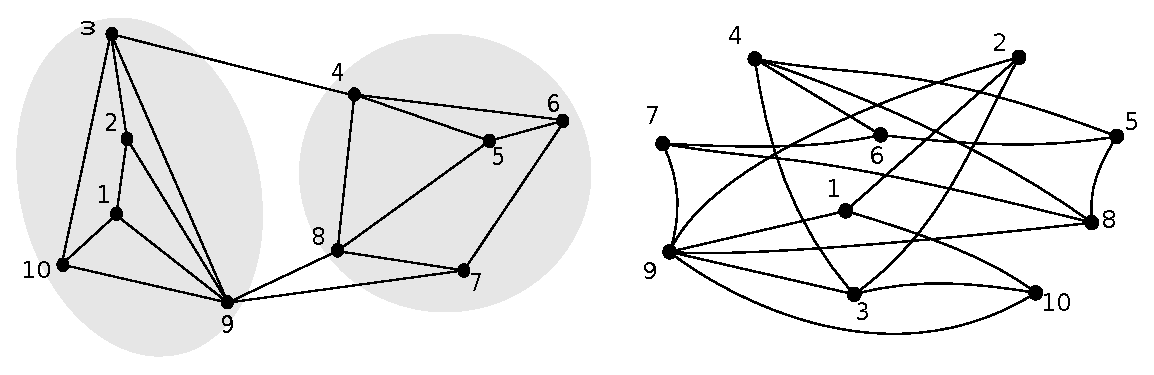
\includegraphics[width=\textwidth]{networkcvsnc.eps}
%  \rule{35em}{0.5pt}
%  \caption{The advantage to clustering a network correctly is seen here.  Both 
%    of these networks have the same nodes and links, and so are the same 
%    network, but they look vastly different because the diagram on the left 
%    has been clustered to maximise modularity.}
%  \label{netclus}
%\end{figure}


\subsection{Newman's Eigenvalue Algorithm}

In \cite{Newman2006a} Newman noted that if we supposed that the network were 
split into two clusters, then we could redefine the modularity in terms of a
quadratic form.  We define a vector $s$, which keeps track of the
split,
$$
s_i = \left\{ \begin{array}{ll} 1 & \mbox{if node $i$ in cluster 1}
  \\ -1 & \mbox{if node $i$ in cluster 2}\end{array} \right.
$$
Then we can redefine modularity as:
\begin{eqnarray}
Q & = & \frac{1}{2m}\sum_{i,j} \left(A_{ij} - \frac{k_ik_j}{2m}\right)\frac{1}{2}(s_is_j + 1)\cr
& = &\frac{1}{4m}\sum_{i,j} \left(A_{ij} - \frac{k_ik_j}{2m}\right)s_is_j,
\end{eqnarray}
Now, if we define a matrix $\mathbf{B}$ where 
$B_{ij} = A_{ij} - k_ik_j/2m$, which we call the {\sl modularity matrix}, 
then we can rewrite this equation as:
\begin{equation}
Q = \frac{1}{4m}{\bf s^tBs}
\end{equation}

Now, since $\mathbf{B}$ is an $n\times n$ symmetric matrix, we know that
it has $n$ real eigenvalues $\lambda_i$, with corresponding
eigenvectors $u_i$.  Now, we order the $\lambda_i$ so that $
\lambda_1 \geq \lambda_2 \geq \ldots \geq \lambda_n$, and we write 
$$
{\bf s} = a_1{\bf u_1}+ \ldots + a_n{\bf u_n}.
$$


The equation for the modularity becomes
\begin{eqnarray}
Q & = & \frac{1}{4m} \sum_{i} a_i{\bf u}_i^t{\bf B}\sum_ja_j{\bf u}_j\cr
& = & \frac{1}{4m} \sum_i \lambda_i ({\bf u}_i^{\bf t}.{\bf s})^2
\end{eqnarray}
so, the positivity of the modularity depends completely on the $\lambda_i$, in 
particular the most positive eigenvalue $\lambda_1$.  This means that to 
maximise the modularity we should take our ``split vector'' $\mathbf{s}$ to be 
as close to the first eigenvector $\mathbf{u}_1$ as possible. To do this, we 
choose $\mathbf{s}$ as follows:

\begin{equation}
s_i =\left\{ \begin{array}{ll} 1 & \mbox{if } u_{1_i}>0 \\
-1 & \mbox{if } u_{1_i}\leq0 \end{array} \right.
\end{equation}

This gives us a clustering of the network into two smaller clusters. Of course, 
this split is not strictly in the direction of $\lambda_1$, but it is our best 
possible estimate\footnote{In fact, it has been noted from well-known networks, 
such as Zachary's karate club \cite{Zachary1977a} that the absolute value of 
the $i$th entry of $\mathbf{u}_1$ gives a good indication of the ``strength'' 
of the membership of node $i$ to its cluster \cite{Newman2006a}.}, given two 
clusters. If the modularity of the split is not positive, then we reject the 
split and say that the best clustering is to leave the network as it is.  
Similarly, if the first eigenvalue $\lambda_1 = 0$ then we say that the best 
clustering is to leave the network undivided, as we know that the modularity 
matrix $\mathbf{B}$ always has a zero eigenvalue, with eigenvector 
$\mathbf{u} = ( 1,1, \ldots, 1)$, which corresponds to no split of the network.

With the network split into two smaller clusters, the next
question is how to split the network further.  We look at the clusters
one-by-one and split them until it gives no benefit to the modularity
of the clustering.  One could naively think that we should look at the
adjacency matrix of the cluster itself, and form the 
corresponding modularity matrix, but this ignores the connectivity of the
overall network.  We could inadvertantly split the subgraph into communities 
which would make sense within the subgraph, but would ignore the connections 
from outside the subgraph. Instead, we need to use the original modularity 
matrix $\mathbf{B}$ and calculate what difference a split of the subgraph would 
make to the modularity.

We call the subgraph $g$ and the {\sl modularity contribution} $\Delta Q$ of a 
split of $g$ is:

\begin{equation}
\Delta Q  =  \frac{1}{2m} \left[ \frac{1}{2}\sum_{i,j\in g}B_{ij}(s_is_j + 1) - \sum_{i,j \in g} B_{ij} \right].
\end{equation}

This is the term in the modularity of the network that a split $\mathbf{s}$ of 
$g$ would change, minus the modularity of leaving the subgraph $g$ whole.  We 
can get our ``subgraph modularity matrix'' $\mathbf{B}^{(g)}$ now:

\begin{samepage}
\begin{eqnarray}
\Delta Q & = & \frac{1}{4m}\left[ \sum_{i,j \in g} B_{ij}s_is_j - \sum_{i,j \in g}B_{ij}\right] \cr
& = & \frac{1}{4m}\sum_{i,j \in g}\left[ B_{ij} - \delta_{ij}\sum_{k \in g} B_{ik}\right]s_is_j \cr
& = & \frac{1}{4m}{\bf s^tB}^{(g)}{\bf s}
\end{eqnarray}
\end{samepage}
and so ${\bf B}^{(g)}$ that takes the value
\begin{equation}
B^{(g)}_{ij} = B_{ij} - \delta_{ij}\sum_{k \in g} B_{ik}
\end{equation}
for labels $i,j$ of nodes in the subgraph $g$.

We can use the same approach as before and find the most
positive eigenvalue of ${\bf B}^{(g)}$ to determine our favoured split
${\bf s}$ to maximise $\Delta Q$. ${\bf B}^{(g)}$ still has the
property that each of its rows and sum to zero, so we still have a
zero-eigenvalue that represents no split of the subgraph.  This can
now be the stopping criterion for the algorithm; if we get a
zero-eigenvalue we say that the subgraph is indivisible and stop
splitting it up.  However, we must be careful that as the most
positive eigenvalue gets smaller, relative to its negative
eigenvalues, there may be no benefit to the modularity of accepting
such a split.  In this case, we check, by calculating $\Delta Q$ for
the proposed split, to see if it is worth continuing splitting the subgraph.
If we get $\Delta Q \leq 0$ then we stop, otherwise we continue
splitting the graph.  The algorithm is summarised in algorithm \ref{algo-split}.

\begin{algorithm}
\caption{This is Newman's eigenvalue algorithm for maximising the modularity of a network.}
\label{algo-split}
\begin{algorithmic}
\STATE Calculate the modularity matrix $\mathbf{B}$, where $B_{ij} = A_{ij} - k_ik_j/2m$
\STATE Find the most positive eigenvalue $\lambda_1$ and its eigenvector $\mathbf{u}_1$
\IF{$\lambda_1 = 0$}
\STATE Stop the algorithm with no split in the network.
\ELSE
\STATE Split network such that node $i$ in first group if $u_{1_{i}} > 0$ and in second group otherwise.
\ENSURE Modularity of split $> 0$
\ENDIF
\FORALL{Subnetworks $g$}
\STATE Calculate $\mathbf{B}^{(g)}$, where $B^{(g)}_{ij} = B_{ij} - \delta_{ij}\sum_{k\in g}B_{ik}$
\STATE Find the most positive eigenvalue $\lambda^{(g)}_1$ of $\mathbf{B}^{(g)}$ and its eigenvector $\mathbf{u}^{(g)}_1$.
\IF{$\lambda^{(g)}_1=0$}
\STATE Subnetwork can split no further.
\ELSE
\STATE Split network such that node $i$ in first group if $u^{(g)}_{1_{i}} > 0$ and in second group otherwise
\ENSURE $\Delta Q > 0$ for split of subnetwork $g$.
\ENDIF
\ENDFOR
\end{algorithmic}
\end{algorithm}



This spectral method for maximising the modularity has shown
remarkably good results \cite{Newman2006a}, in fact considerably better results
than the {\sl betweenness} algorithm of Newman and Girvan 
\cite{NewmanGirvan2004a}, despite the apparent drawback of always splitting the 
network/subgraph in two parts. It is also possible to use the first $m$ 
eigenvalues and use the $i$th entry of the eigenvectors as coordinates in 
$\mathbf{R}^{m}$ \cite{Humphries2011a}, but this then requires a choice of 
number of clusters, which may not be known from the data.  This may also 
require calculating many more eigenvalues of the large matrix $\mathbf{B}$, 
which can be computationally expensive.  I plan to try and implement a similar 
algorithm using the first two eigenvectors, $\lambda_1$ and $\lambda_2$, as 
coordinates in $\mathbf{R}^2$ and using $k$-means clustering on the projections 
of these coordinates on $S^1$.  This method will of course lead to greater 
computation times, but it should hopefully resolve some of the problems of 
splitting the network in two, without becoming completely prohibitive 
computationally.

\section{Spike Trains}

Neurons convey information through the nervous system by generating
electric pulses which propagate along nerve fibers.  These pulses are
called action potentials or spikes \cite{DayanAbbott2001a}. 

A neuron has a resting potential of approximately -70mV relative to
its surroundings, and we say that the cell is polarised at this point.
The membrane potential of a neuron becomes less negative with current
flowing into it, but will tend back towards its resting potential
unless the membrane potential nears a certain threshold. If a neuron
is depolarised so that its membrane potential is raised above this
threshold, the neuron generates an action potential. An action potential, or 
spike, is a 100mV fluctuation in the membrane potential which lasts 
approximately 1ms. Following the production of a spike the neuron briefly 
becomes hyperpolarised, and as such cannot generate a spike for the next
couple of milliseconds.  This period, when a spike cannot be fired, is
called the absolute refractory period of a neuron.  Since the neuron
becomes hyperpolarised by the spike, there is also a period in which
it is ``more difficult'' for the neuron to spike again, this is called
the relative refractory period of a neuron. 

Spikes are very important because they propagate over long distances without 
attenuation, and so are the way in which neurons communicate with one another 
throughout the nervous system.  The timing of spikes is of particular 
importance; for example, in motor neurons when a number of spikes happen close 
together it leads to movement of the muscle, the more spikes that happen 
together, the faster the muscle twitches.  While there is some variation in 
the duration, amplitude and shape of action potentials, we can largely treat 
them as identical processes, where the timing is the only consideration.  So, 
if a neuron spikes $n$ times in a certain trial, then the trial can be 
described by the times of the spikes $t_i$.  Then we can describe the 
{\sl spike train} mathematically as:

\begin{equation}
s(t) = \sum_{i=1}^n \delta(t-t_i).
\end{equation}
The $\delta$ here is the Dirac delta, which essentially gives a spike of volume 
one at the point $t_i$. It can be very difficult to differentiate between 
different spike trains, and so we have {\sl metrics} to tell them apart.

\subsection{Spike Train Metrics}

If we look at spike trains from a specific neuron, we would like to be able to 
``decode'' them and be able to describe the stimulus which evoked them.  
Unfortunately, this seems like a very difficult problem, so we first settle for 
trying to distinguish which spike trains amongst a collection were evoked by 
the same stimulus.  To do this, there are several {\sl metrics} in the 
literature which tell us the ``distance'' between two spike trains.  

In Mathematics a metric space is a space where we can always tell the 
``distance'' between two elements, whether or not we can give the 
``coordinates'' of the elements in the space.  A metric is a function on a set 
$X$, $d: X\times X \rightarrow [0,\infty )$ that basically follows our 
intuition for what a distance should be. That is, distances are non-negative, 
symmetric and only zero if two elements are the same. The Triangle Inequality 
states that you should never be able to shorten the distance between two points 
by going through an intermediate point, so it is the notion that the shortest 
distance between two points is a straight line.


\subsection{Van Rossum metric}

The metric that we primarily use is the metric described by van Rossum in 
\cite{VanRossum2001a}, which is simply based on the $L^2$ metric on function 
spaces.  If we view the spike trains as a collection of Dirac delta functions, 
then we can get a function by convolving the distribution $s(t)$ as above with 
a kernel.  A common kernel that is used is the exponential kernel 
\begin{equation}
k(t) = \left\{ \begin{array}{ll}\frac{1}{\tau}e^{-\frac{t}{\tau}}, & t\geq 0 \\
0, & t<0\end{array} \right. .
\end{equation}

This kernel has some advantages, like causality and computability, over a 
gaussian kernel.  So, we get a new function $u(t)$ after convolving the spike 
train with the kernel:
\begin{equation}
u(t) = s*k(t) = \int_0^T s(t-s)k(s)\,ds
\end{equation}



%\begin{figure}[tb]
%  \centering
%  \includegraphics[width=0.8\textwidth]{spiketrainkernel.eps}
%  \rule{35em}{0.5pt}
%  \caption{This figure shows  an exponential kernel (a), which we convolve with a spike train (b), to get the function (c) which represents the spike train.  We take the  $L^2$-metric between such functions to get the van Rossum metric between spike trains.}
%  \label{stk}
%\end{figure}

Figure \ref{stk} above shows the form of the function that we get when we 
convolve a spike train with the exponential kernel.  Once we have these 
functions for different spike trains, $u$ and $v$ say, then we calculate the 
distance between them by taking the $L^2$ metric on the function space, that is:

\begin{equation}
d(u,v) = \sqrt{\int_0^T (u(t) - v(t))^2\,dt}
\end{equation}



This metric has some mathematical advantages over other metrics, such as Victor-
Purpura \cite{VictorPurpura1997a}, an ``edit-length'' metric, because there is 
a lot of material in functional analysis on the $L^2$ metric.  It performs to a 
similar standard to most other metrics, and remarkably the choice of kernel has 
little effect on its efficiency.


\subsection{$k$-Medoids Clustering}

By defining a metric on spike trains, we can tell how close different responses 
are to each other, but there are no ``co-ordinates'' in the metric space which 
would help with clustering responses.  The standard method of clustering 
spike-trains is similar to $k$-means clustering, but since there is no standard 
method for computing a ``mean spike-train'' given a number of spike trains, it 
must be altered slightly.

For $k$-means clustering, we select $k$ random points in the space in which 
clustering is occuring, then each point in the space would be in the cluster of 
the closest of these $k$ points to itself.  Then we would find the mean of all 
the points in a cluster to get a new ``centre'' for the cluster and re-cluster 
each point to the closest of these $k$ means.  This process is repeated until 
the means are stable, which gives a clustering of the points into $k$ clusters.

Unfortunately, since there is no mean in the metric space of spike-trains, we 
cannot perform $k$-means clustering, rather, we perform $k$-medoids.  In 
$k$-medoids, we randomly choose $k$ points in the data, which we call medoids, 
and then we place each other point of the data in the cluster of the 
``closest'' (or, least dissimilar) medoid to it.  Then, for each cluster, we 
swap the medoid for each other point in the cluster, and choose the one with 
the least overall distance as the new medoid. This step is shown in Figure 
\ref{kmed} below. We repeat these steps until there is no change in the 
medoids.  This method suits us for spike-trains, as the idea of a ``mean'' 
spike-train is not well understood, but there is currently a very promising 
method proposed by other members of this lab, which is to be submitted shortly.

There are some downsides to using $k$-medoids, that I hoped could possibly be 
improved by using network methods.  The primary disadvantage is that you must 
select how many clusters in advance, and hence you must know how many different 
stimuli were used when you look at a data set.  The next chapter deals with our 
efforts to address this issue.

%\begin{figure}[t]
%  \centering
%  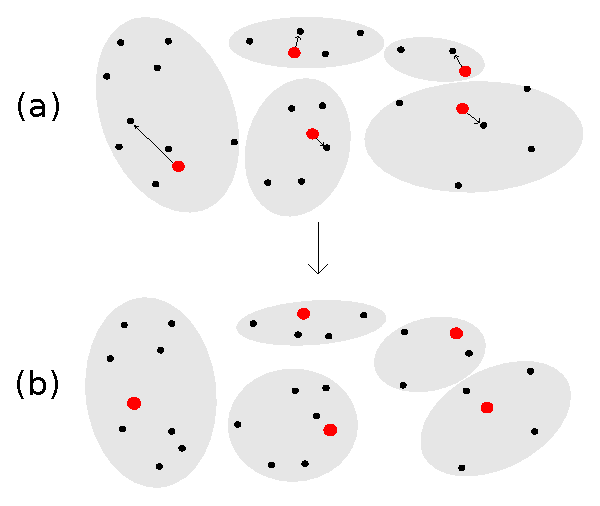
\includegraphics[width=0.8\textwidth]{kmedoids.eps}
%  \rule{35em}{0.5pt}
%  \caption{An example of the first step in k-medoids clustering:  (a) Medoids 
%    are initially selected at random and the first clustering puts each point 
%    in the cluster of the closest medoid. Then we choose the point in the 
%    cluster that will give the lowest total distance to other points, and 
%    choose that as the new medoid. (b) Finally, we re-cluster each point to go 
%    in the cluster of the closest medoid to it.}
%  \label{kmed}
%\end{figure}

\subsection{Clustering Responses with Modularity}


We proposed that we could perhaps improve on current methods of sorting 
responses by using the modularity clustering algorithm.  The advantage to such 
a method would be that we would hopefully not need to know how many different 
stimuli there were. Since the algorithm determines when to stop itself, it 
could simply be run to completion.  Such a method could perhaps be used for 
many different data sets, when the number of stimuli was not known, to 
determine the different responses.

We used the data set from \cite{NarayanEtAl2006b}, which featured spike trains 
from anesthetized adult male zebra finches as they listened to natural 
birdsong.  Each neuron was played $20$ songs ten times each, so we had $200$ 
data points from which to form a network for each neuron.

We formed a network by first taking the Van-Rossum metric distances between 
each pair of responses, then we chose a threshold value $\tau$ for the network 
and we set

\begin{equation}
A^{\tau}_{ij} = \left\{ \begin{array}{ll} 1 & \mbox{if }d(i,j)<\tau \\
0 & \mbox{otherwise}
\end{array}\right. .
\end{equation}

Once we have the adjacency matrix for our network, we can run the algorithm to 
maximise modularity for the network.  For the data that we used, 
each spike train was less than a second long, so the maximum Van Rossum 
distance between any two trains was one, so we ran the algorithm for different 
threshold values $\tau$ between zero and one incrementing $\tau$ by steps of 
size $0.001$.

As we can see in Figure \ref{graphs}, the profile of the graph of the maximum 
modularity versus the threshold looked promising, as in nearly all cases it had 
a clear maximum, but unfortunately the clusters of responses bore little 
resemblance to the stimuli, and usually had too few clusters.

%\begin{figure}[thb]
%  \centering
%  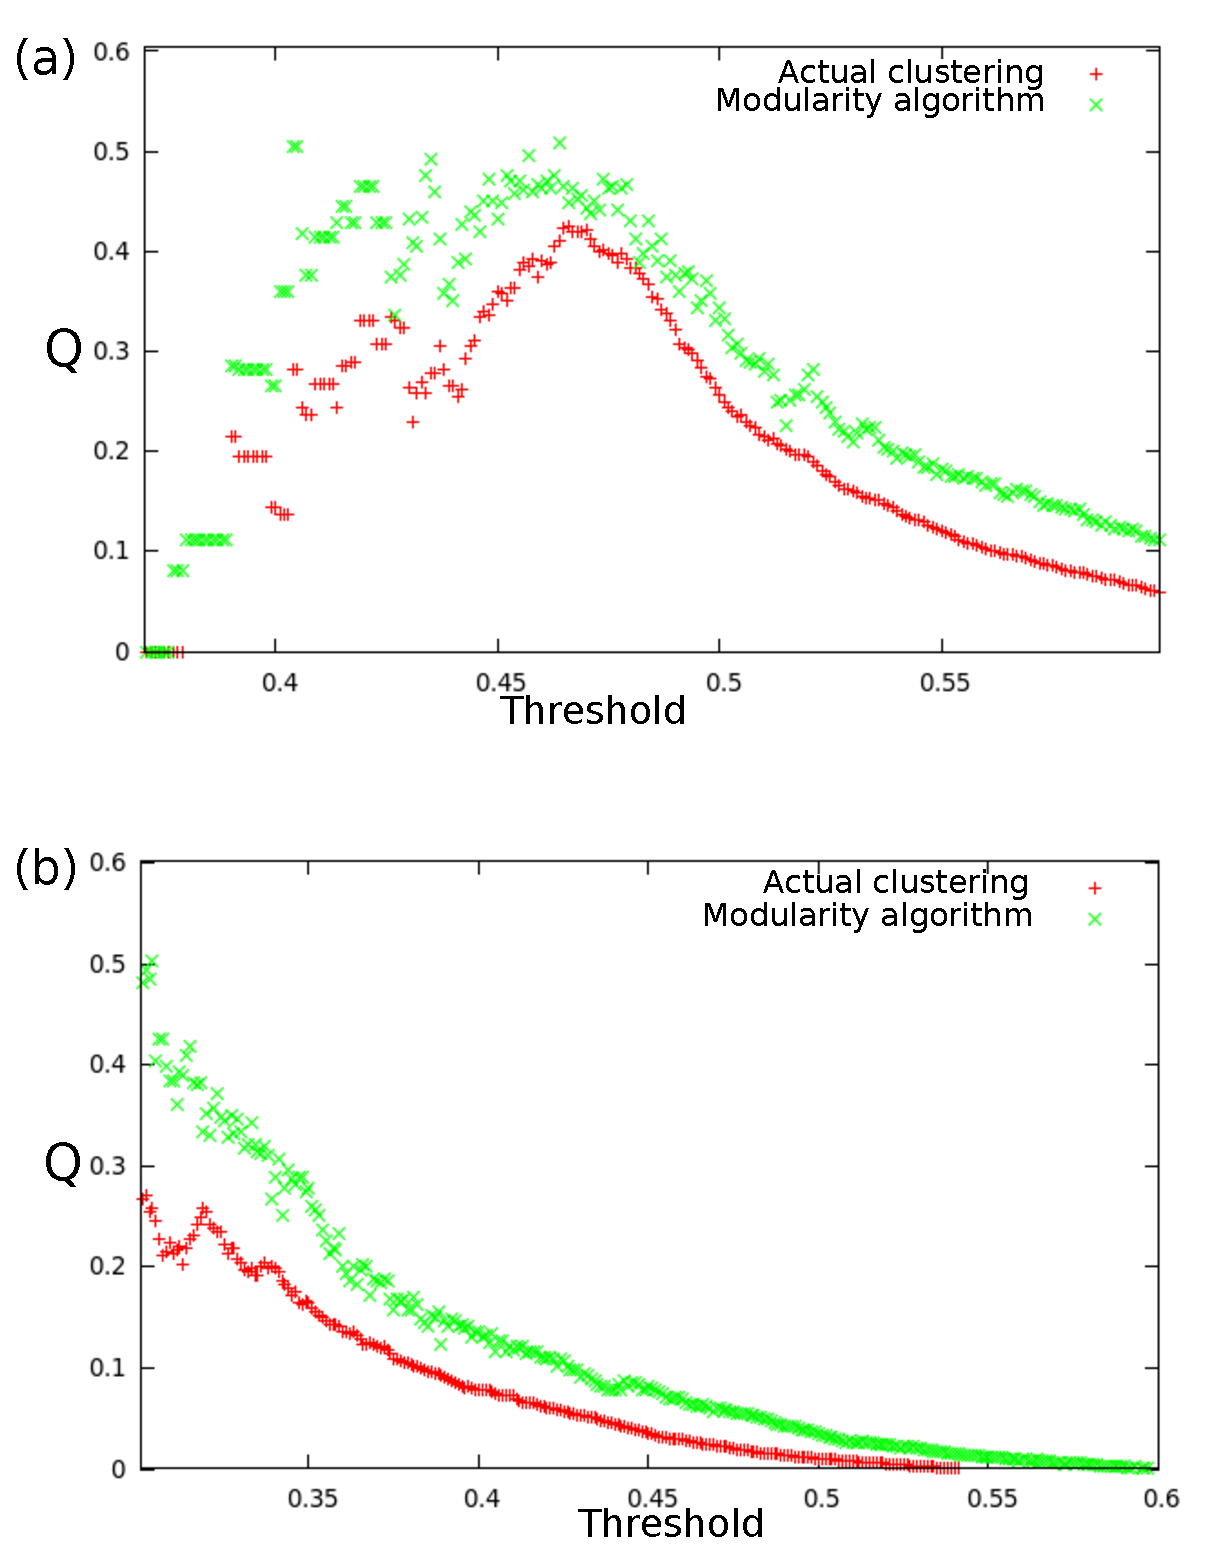
\includegraphics[width=0.8\textwidth]{expresults.eps}
%  \rule{35em}{0.5pt}
%  \caption{Above you can see the graph of the modularity versus threshold values
%    in two typical cells from the data.  The green crosses represent the 
%    modularity of the correct clustering of stimuli; the red plusses represent 
%    the maximum modularity, according to the algorithm, of the network.
%    Despite there being clear peaks in the graphs, we see that the green 
%    consistently outperforms the red for every value of the threshold $\tau$.  
%    This seems to imply that network clustering methods are probably not very 
%    good for sorting stimuli.}
%  \label{graphs}
%\end{figure}

It appears that the margins are just too small, and there is no natural 
network, rather a bunch of networks determined by a strict cut-off, so the 
modularity algorithm cuts some of the correct clusters in two.  A recent paper 
by Humphries \cite{Humphries2011a} uses all of the positive eigenvalues to 
cluster the responses with more accuracy. This method is 
rather computationally expensive, and uses even the very small positive 
eigenvaluse, which tell us very little about the positivity of modularity, so 
we tried to use Newman's more simple algorithm, despite its obvious drawbacks.

The thing that was most disappointing was that the correct clustering nearly 
always gave a lower modularity than the algorithm, so it seems like network 
clustering methods just may not be very useful for this problem.


\section{Discussion}
Due to the fact that the modularity that the algorithm found for the network is 
higher than the modularity of the correct clustering, it is clear that network 
methods are not useful to sort stimuli from a single neuron.  Since the 
original goal was to illuminate the functionality of the brain, or at least 
small areas of the brain, this non-result doesn't matter too much.  We want to 
get simultaneous recordings from many neurons, and form networks which would 
correspond to different neurons rather than spike trains.

There are different ways to form the networks of many neurons, but we will 
mainly be interested in neurons that seem to {\sl drive} other neurons.  That 
is, neurons whose firing seems to improve the probability of the other neuron 
firing significantly.  A method that particularly interests us is the method of 
{\sl Incremental Mutual Information} of Singh and Lesica 
\cite{SinghLesica2010a}, which tries to reduce the uncertainty of a neuron as 
much as possible before checking whether another neuron influences it.

Any network formed from this measure would have to be directed, so we need a 
method to turn a directed network into an undirected network.  Newman describes 
a very neat way to do this in \cite{Newman2010a}, where two nodes are related 
in the undirected network by how many commons nodes they point to in the 
directed network.  He calls this the {\sl bibliographic coupling} of two 
nodes.  In a brain network, this could give us a ``map'' of information flow.

Once we have our new networks, we may use some other network measures to 
examine them as in \cite{RubinovSporns2010a}.  The {\sl clustering coefficient} 
is a useful local measure for how clustered a node is, and it may be useful to 
use this along with the modularity to find and study community structure.



\chapter{Multi-unit spike train metrics}
The SPIKE distance proposed by Kreuz et al in \cite{Kreuzetal2010} is an instantaneous parameter-free distance measure between spike-trains.  By instantaneous measure, it is meant that for each time $t$ there is a time-local distance between two spike-trains.  This measure can the be integrated over the length of the spike-trains to give a parameter-free distance measure between spike trains. In the study of spike-train metrics, often a multi-unit measure is desired (to minimise compounding any errors that may result from inefficient spike-sorting?). A multi-unit measure is a distance between collections of labelled spike-trains.  The SPIKE distance in \cite{Kreuzetal2010} does not lend itself to a simple multi-unit extension, so instead a simpler version of the SPIKE distance is extended.

\section{Single-unit recordings}
With a view to extending the SPIKE distance to a multi-unit distance measure, it is useful to review the definition of the SPIKE measure provided in \cite{Kreuzetal2010}:  Given two spike-trains $x$ and $y$, where $x = \{ t_1^x, \ldots, t_n^x \}$ and $y = \{ t_1^y, \ldots , t_m^y\}$, where $t_1^x,\ldots,t_n^x,t_1^y,\ldots,t_m^y$ are the spike times.  The SPIKE distance in \cite{Kreuzetal2010} has the nice property that the distance is bounded such that it is always between zero and one.  Unfortunately, to achieve a ``natural�� extension to a multi-unit measure, this property is sacrificed.  A simpler version of the distance, without the strict upper bound of one, is used.

The simpler distance is very quick and easy to calculate.  A `gap� is associated with each spike; this is the distance to the nearest spike in the other spike-train.  The total distance between two spike trains is then the sum of these gaps.  The original SPIKE distance included additional normalisation factors that have been omitted in simplifying the measure.  To form the time-local distance, a weighted sum of the gaps for the corner spikes is made, that is, the spikes preceding and following the time of interest in each of the two spike trains.  The weighting is chosen so that the integral of the time-local function is just the sum of the gaps.

First, the gaps are calculated for each spike in the two spike-trains.  This is simply the nearest spike in the other spike train:
\begin{equation}
\Delta t_i^x = min_i ( | t_i^x - t_i^y |)
\end{equation}
At each time instant, these is a unique set of four corner spikes: the preceding and following spikes from each spike train, which are labelled $t_P^x(t), t_F^x(t), t_P^y(t)$ and  $t_F^y(t)$; these are, respectively, the preceding and following spikes in spike-train $x$ and the preceding and following spikes in spike-train $y$.

For each spike-train, w, a time-local distance is then calculated using the associated gap of the four corner spikes for each spike-train, $w=x,y$:
\begin{equation}
s_w(t) = \frac{\lambda_P(t) \Delta t_P^w(t) + \lambda_F(t)\Delta t_F^w(t)}{I^w(t)}
\end{equation}
where
\begin{equation}
\lambda_F^w(t) = \frac{t- t_P^w(t)}{I^w(t)}, \, \lambda_P^w(t) = \frac{ t_F^w(t) - t}{I^w(t)}
\end{equation}
and $I^w(t)$ is the size of the interval in which $t$ is contained:
\begin{equation}
I^w(t) = t_F^w(t) - t_P^w(t).
\end{equation}
Now, the time-local distance for each neuron is added to give the overall time-local distance:
\begin{equation}
s(t) = s_x(t) + s_y(t).
\end{equation}

This simplified time-local SPIKE distance has the advantage that its integral is simply the sum of the gaps of each spike; that is:
\begin{equation}
\int_0^T s(t)\, dt = \sum_w \sum_i \Delta t_i^w.
\end{equation}

In practice this simplified version of SPIKE produces similar time profiles to the version described in \cite{Kreuzetal2010}. The time-local distance profile for two similar spike-trains is given in Figure [NEED TO ADD PICTURE].

\section{Extension to multi-unit recordings}

\chapter{A simple neuron model}
Sparse coding has been observed in neurons in the visual tract \cite{OlshausenField2004}, a simple model is proposed for such neurons.

It is unlikely that a neuron is ever truly ``off��, so it is assumed that a neuron has a base-firing state that will be referred to as the ``off-state��.  For the sake of simplicity, it is assumed that a neuron in such an ``off-state�� would have a constant firing rate, $\lambda_d$.  Correspondingly, for sparse-coding a neuron must have a higher firing-rate when the feature that it codes for is present; this firing rate, $\lambda_u$, is also taken to be constant.

The model also assumes that the

\chapter{Conclusion}
In chapter two of this thesis, clustering methods of network theory were used to attempt to address several problems.  

Initially, there was an attempt to cluster responses by forming a network based on the distance between them, using the van Rossum metric. The clustering algorithms did not separate responses into the correct stimuli particularly well.  This is likely due to the unnatural structure of the network.  Spike train metrics are affected by the noise in the system, and so a responses that is \lq{}close\rq{} may not have a significantly different metric value to one that is not.  A study of baseline expected values of spike train metrics could lead to a better representative network of responses.

The incremental mutual information of \citep{SinghLesica2010a} proved to be a very useful tool to actually determine direction of influence between neurons in a network.  It would, however, be very difficult to collect data sets that are long enough to fully determine the probability spaces.  This is always a problem with any information theory measure, due to the fact that there are no assumptions made about the prior probability distributions.

The bibliographic coupling and cocitation did cluster the network into cooperative groups, but could not completely accurately describe the diagram of the model network.  There may be a way to combine the two couplings to do so, but any method of combining the maximum or the mean of the couplings did not prove to work for the model used in this work. 

In chapter three, several extensions of distance measures were provided to the SPIKE and the ISI distances from \citep{KreuzEtAl2007a,KreuzEtAl2012a}. These extensions proved to be comparable to the multi-unit extensions to the Victor-Purpura metric \citep{AronovEtAl2008a} and the van Rossum metric \citep{HoughtonSen2008a}.

The multi-unit ISI extensions lead to a different understanding of the summed population codes.  This motivated the search for the background rate which Chapter Four was centred on.

The firing model introduced was very simplistic, but it was based on the fact that neurons are often feature-specific.  That assumption suggested that there should be a bimodality in the firing rates of a neuron.

The bimodal firing rate suggest that the ISI distribution of the neuron should be a hyperexponential distribution, with two time-scales, rather than an exponential distribution.  When this distribution was tested on the data, it significantly out-performed the exponential distribution, and adding a third mode did not improve results.  Thus, it seems as though neurons should have this \lq{}on-off\rq{} firing rate.



\bibliography{bibliography}

\end{document}